% Created by tikzDevice version 0.10.1 on 2016-08-15 14:59:40
% !TEX encoding = UTF-8 Unicode
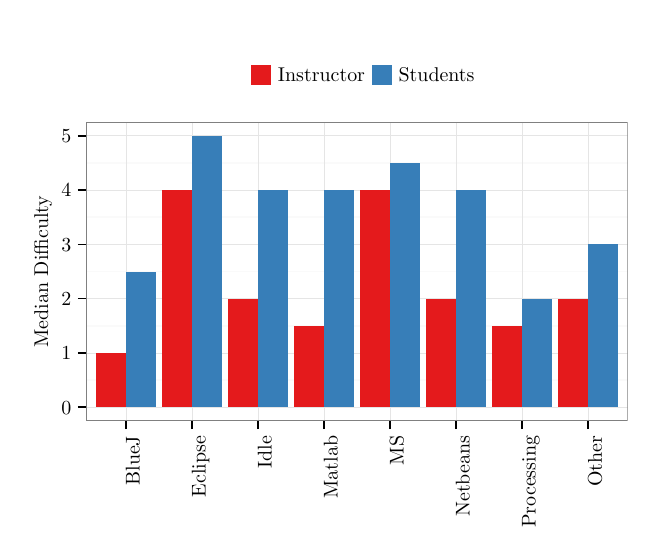
\begin{tikzpicture}[x=1pt,y=1pt]
\definecolor{fillColor}{RGB}{255,255,255}
\path[use as bounding box,fill=fillColor,fill opacity=0.00] (0,0) rectangle (216.81,180.67);
\begin{scope}
\path[clip] (  0.00,  0.00) rectangle (216.81,180.67);
\definecolor{drawColor}{RGB}{255,255,255}
\definecolor{fillColor}{RGB}{255,255,255}

\path[draw=drawColor,line width= 0.6pt,line join=round,line cap=round,fill=fillColor] ( -0.00,  0.00) rectangle (216.81,180.68);
\end{scope}
\begin{scope}
\path[clip] ( 21.16, 38.59) rectangle (216.81,146.53);
\definecolor{fillColor}{RGB}{255,255,255}

\path[fill=fillColor] ( 21.16, 38.59) rectangle (216.81,146.53);
\definecolor{drawColor}{gray}{0.98}

\path[draw=drawColor,line width= 0.6pt,line join=round] ( 21.16, 53.31) --
	(216.81, 53.31);

\path[draw=drawColor,line width= 0.6pt,line join=round] ( 21.16, 72.94) --
	(216.81, 72.94);

\path[draw=drawColor,line width= 0.6pt,line join=round] ( 21.16, 92.56) --
	(216.81, 92.56);

\path[draw=drawColor,line width= 0.6pt,line join=round] ( 21.16,112.19) --
	(216.81,112.19);

\path[draw=drawColor,line width= 0.6pt,line join=round] ( 21.16,131.81) --
	(216.81,131.81);
\definecolor{drawColor}{gray}{0.90}

\path[draw=drawColor,line width= 0.2pt,line join=round] ( 21.16, 43.50) --
	(216.81, 43.50);

\path[draw=drawColor,line width= 0.2pt,line join=round] ( 21.16, 63.12) --
	(216.81, 63.12);

\path[draw=drawColor,line width= 0.2pt,line join=round] ( 21.16, 82.75) --
	(216.81, 82.75);

\path[draw=drawColor,line width= 0.2pt,line join=round] ( 21.16,102.37) --
	(216.81,102.37);

\path[draw=drawColor,line width= 0.2pt,line join=round] ( 21.16,122.00) --
	(216.81,122.00);

\path[draw=drawColor,line width= 0.2pt,line join=round] ( 21.16,141.63) --
	(216.81,141.63);

\path[draw=drawColor,line width= 0.2pt,line join=round] ( 35.47, 38.59) --
	( 35.47,146.53);

\path[draw=drawColor,line width= 0.2pt,line join=round] ( 59.33, 38.59) --
	( 59.33,146.53);

\path[draw=drawColor,line width= 0.2pt,line join=round] ( 83.19, 38.59) --
	( 83.19,146.53);

\path[draw=drawColor,line width= 0.2pt,line join=round] (107.05, 38.59) --
	(107.05,146.53);

\path[draw=drawColor,line width= 0.2pt,line join=round] (130.91, 38.59) --
	(130.91,146.53);

\path[draw=drawColor,line width= 0.2pt,line join=round] (154.77, 38.59) --
	(154.77,146.53);

\path[draw=drawColor,line width= 0.2pt,line join=round] (178.63, 38.59) --
	(178.63,146.53);

\path[draw=drawColor,line width= 0.2pt,line join=round] (202.49, 38.59) --
	(202.49,146.53);
\definecolor{fillColor}{RGB}{55,126,184}

\path[fill=fillColor] ( 35.47, 43.50) rectangle ( 46.21, 92.56);
\definecolor{fillColor}{RGB}{228,26,28}

\path[fill=fillColor] ( 24.74, 43.50) rectangle ( 35.47, 63.12);
\definecolor{fillColor}{RGB}{55,126,184}

\path[fill=fillColor] ( 59.33, 43.50) rectangle ( 70.07,141.63);
\definecolor{fillColor}{RGB}{228,26,28}

\path[fill=fillColor] ( 48.60, 43.50) rectangle ( 59.33,122.00);
\definecolor{fillColor}{RGB}{55,126,184}

\path[fill=fillColor] ( 83.19, 43.50) rectangle ( 93.93,122.00);
\definecolor{fillColor}{RGB}{228,26,28}

\path[fill=fillColor] ( 72.46, 43.50) rectangle ( 83.19, 82.75);
\definecolor{fillColor}{RGB}{55,126,184}

\path[fill=fillColor] (107.05, 43.50) rectangle (117.79,122.00);
\definecolor{fillColor}{RGB}{228,26,28}

\path[fill=fillColor] ( 96.32, 43.50) rectangle (107.05, 72.94);
\definecolor{fillColor}{RGB}{55,126,184}

\path[fill=fillColor] (130.91, 43.50) rectangle (141.65,131.81);
\definecolor{fillColor}{RGB}{228,26,28}

\path[fill=fillColor] (120.18, 43.50) rectangle (130.91,122.00);
\definecolor{fillColor}{RGB}{55,126,184}

\path[fill=fillColor] (154.77, 43.50) rectangle (165.51,122.00);
\definecolor{fillColor}{RGB}{228,26,28}

\path[fill=fillColor] (144.04, 43.50) rectangle (154.77, 82.75);
\definecolor{fillColor}{RGB}{55,126,184}

\path[fill=fillColor] (178.63, 43.50) rectangle (189.37, 82.75);
\definecolor{fillColor}{RGB}{228,26,28}

\path[fill=fillColor] (167.90, 43.50) rectangle (178.63, 72.94);
\definecolor{fillColor}{RGB}{55,126,184}

\path[fill=fillColor] (202.49, 43.50) rectangle (213.23,102.37);
\definecolor{fillColor}{RGB}{228,26,28}

\path[fill=fillColor] (191.76, 43.50) rectangle (202.49, 82.75);
\definecolor{drawColor}{gray}{0.50}

\path[draw=drawColor,line width= 0.6pt,line join=round,line cap=round] ( 21.16, 38.59) rectangle (216.81,146.53);
\end{scope}
\begin{scope}
\path[clip] (  0.00,  0.00) rectangle (216.81,180.67);
\definecolor{drawColor}{RGB}{0,0,0}

\node[text=drawColor,anchor=base east,inner sep=0pt, outer sep=0pt, scale=  0.72] at ( 15.76, 41.02) {0};

\node[text=drawColor,anchor=base east,inner sep=0pt, outer sep=0pt, scale=  0.72] at ( 15.76, 60.64) {1};

\node[text=drawColor,anchor=base east,inner sep=0pt, outer sep=0pt, scale=  0.72] at ( 15.76, 80.27) {2};

\node[text=drawColor,anchor=base east,inner sep=0pt, outer sep=0pt, scale=  0.72] at ( 15.76, 99.90) {3};

\node[text=drawColor,anchor=base east,inner sep=0pt, outer sep=0pt, scale=  0.72] at ( 15.76,119.52) {4};

\node[text=drawColor,anchor=base east,inner sep=0pt, outer sep=0pt, scale=  0.72] at ( 15.76,139.15) {5};
\end{scope}
\begin{scope}
\path[clip] (  0.00,  0.00) rectangle (216.81,180.67);
\definecolor{drawColor}{RGB}{0,0,0}

\path[draw=drawColor,line width= 0.6pt,line join=round] ( 18.16, 43.50) --
	( 21.16, 43.50);

\path[draw=drawColor,line width= 0.6pt,line join=round] ( 18.16, 63.12) --
	( 21.16, 63.12);

\path[draw=drawColor,line width= 0.6pt,line join=round] ( 18.16, 82.75) --
	( 21.16, 82.75);

\path[draw=drawColor,line width= 0.6pt,line join=round] ( 18.16,102.37) --
	( 21.16,102.37);

\path[draw=drawColor,line width= 0.6pt,line join=round] ( 18.16,122.00) --
	( 21.16,122.00);

\path[draw=drawColor,line width= 0.6pt,line join=round] ( 18.16,141.63) --
	( 21.16,141.63);
\end{scope}
\begin{scope}
\path[clip] (  0.00,  0.00) rectangle (216.81,180.67);
\definecolor{drawColor}{RGB}{0,0,0}

\path[draw=drawColor,line width= 0.6pt,line join=round] ( 35.47, 35.59) --
	( 35.47, 38.59);

\path[draw=drawColor,line width= 0.6pt,line join=round] ( 59.33, 35.59) --
	( 59.33, 38.59);

\path[draw=drawColor,line width= 0.6pt,line join=round] ( 83.19, 35.59) --
	( 83.19, 38.59);

\path[draw=drawColor,line width= 0.6pt,line join=round] (107.05, 35.59) --
	(107.05, 38.59);

\path[draw=drawColor,line width= 0.6pt,line join=round] (130.91, 35.59) --
	(130.91, 38.59);

\path[draw=drawColor,line width= 0.6pt,line join=round] (154.77, 35.59) --
	(154.77, 38.59);

\path[draw=drawColor,line width= 0.6pt,line join=round] (178.63, 35.59) --
	(178.63, 38.59);

\path[draw=drawColor,line width= 0.6pt,line join=round] (202.49, 35.59) --
	(202.49, 38.59);
\end{scope}
\begin{scope}
\path[clip] (  0.00,  0.00) rectangle (216.81,180.67);
\definecolor{drawColor}{RGB}{0,0,0}

\node[text=drawColor,rotate= 90.00,anchor=base east,inner sep=0pt, outer sep=0pt, scale=  0.72] at ( 40.43, 33.19) {BlueJ};

\node[text=drawColor,rotate= 90.00,anchor=base east,inner sep=0pt, outer sep=0pt, scale=  0.72] at ( 64.29, 33.19) {Eclipse};

\node[text=drawColor,rotate= 90.00,anchor=base east,inner sep=0pt, outer sep=0pt, scale=  0.72] at ( 88.15, 33.19) {Idle};

\node[text=drawColor,rotate= 90.00,anchor=base east,inner sep=0pt, outer sep=0pt, scale=  0.72] at (112.01, 33.19) {Matlab};

\node[text=drawColor,rotate= 90.00,anchor=base east,inner sep=0pt, outer sep=0pt, scale=  0.72] at (135.87, 33.19) {MS};

\node[text=drawColor,rotate= 90.00,anchor=base east,inner sep=0pt, outer sep=0pt, scale=  0.72] at (159.73, 33.19) {Netbeans};

\node[text=drawColor,rotate= 90.00,anchor=base east,inner sep=0pt, outer sep=0pt, scale=  0.72] at (183.59, 33.19) {Processing};

\node[text=drawColor,rotate= 90.00,anchor=base east,inner sep=0pt, outer sep=0pt, scale=  0.72] at (207.45, 33.19) {Other};
\end{scope}
\begin{scope}
\path[clip] (  0.00,  0.00) rectangle (216.81,180.67);
\definecolor{drawColor}{RGB}{0,0,0}

\node[text=drawColor,rotate= 90.00,anchor=base,inner sep=0pt, outer sep=0pt, scale=  0.72] at (  7.36, 92.56) {Median Difficulty};
\end{scope}
\begin{scope}
\path[clip] (  0.00,  0.00) rectangle (216.81,180.67);
\definecolor{fillColor}{RGB}{255,255,255}

\path[fill=fillColor] ( 72.21,155.07) rectangle (165.76,172.14);
\end{scope}
\begin{scope}
\path[clip] (  0.00,  0.00) rectangle (216.81,180.67);
\definecolor{fillColor}{RGB}{228,26,28}

\path[fill=fillColor] ( 80.80,160.05) rectangle ( 87.92,167.16);
\end{scope}
\begin{scope}
\path[clip] (  0.00,  0.00) rectangle (216.81,180.67);
\definecolor{fillColor}{RGB}{55,126,184}

\path[fill=fillColor] (124.42,160.05) rectangle (131.54,167.16);
\end{scope}
\begin{scope}
\path[clip] (  0.00,  0.00) rectangle (216.81,180.67);
\definecolor{drawColor}{RGB}{0,0,0}

\node[text=drawColor,anchor=base west,inner sep=0pt, outer sep=0pt, scale=  0.72] at ( 90.43,161.12) {Instructor};
\end{scope}
\begin{scope}
\path[clip] (  0.00,  0.00) rectangle (216.81,180.67);
\definecolor{drawColor}{RGB}{0,0,0}

\node[text=drawColor,anchor=base west,inner sep=0pt, outer sep=0pt, scale=  0.72] at (134.06,161.12) {Students};
\end{scope}
\end{tikzpicture}
